\documentclass[10pt,a4paper]{article}
\usepackage[utf8]{inputenc}
\usepackage[spanish]{babel}
\usepackage{amsmath}
\usepackage{amsfonts}
\usepackage{amssymb}
\usepackage{float}
\usepackage{graphicx}
\usepackage[left=2cm,right=2cm,top=2cm,bottom=2cm]{geometry}

\begin{document}
\section{Parte 3}
Se pidió desarrollar un programa con interfaz gráfica de usuario, cuyo propósito fuera el de facilitar la confección de gráficos, mediante un método de ploteo automático. El programa debe implementarse en Python, y debe cumplir con los siguientes requisitos básicos. 
En primer lugar, respecto a fuentes desde las cuales se puede ingresar datos a graficar, los mismos deben ser:
\begin{itemize}
\item Función transferencia
\item Archivo LTspice
\item Plantilla de Excel o csv con mediciones
\end{itemize}
En segundo lugar, se de debe otorgar al usuario las siguientes capacidades:
\begin{itemize}
\item Especificar la etiqueta para el eje x.
\item Especificar la etiqueta para el eje y.
\item Guardar el gráfico como imagen.
\item Borrar todos los gráficos anteriores.
\item Graficar más de tres señales simultáneamente.
\end{itemize}

\subsection{Guía de usuario}
A continuación se explicará detalladamente cada paso referente a la utilización de la GUI implementada. Los pasos a desarrollar son el ingreso de datos desde los distintos tipos de fuentes, edición de las etiquetas, seleccionar la visualización del gráfico en una o dos figuras, eliminar los gráficos anteriores y por ultimo, la exportación de los gráficos.

Previo a desarrollar los pasos se muestra una figura con el diseño de la interfaz gráfica, tal cual se muestra una vez que el usuario inicia el programa

\begin{figure}[ht]
\centering
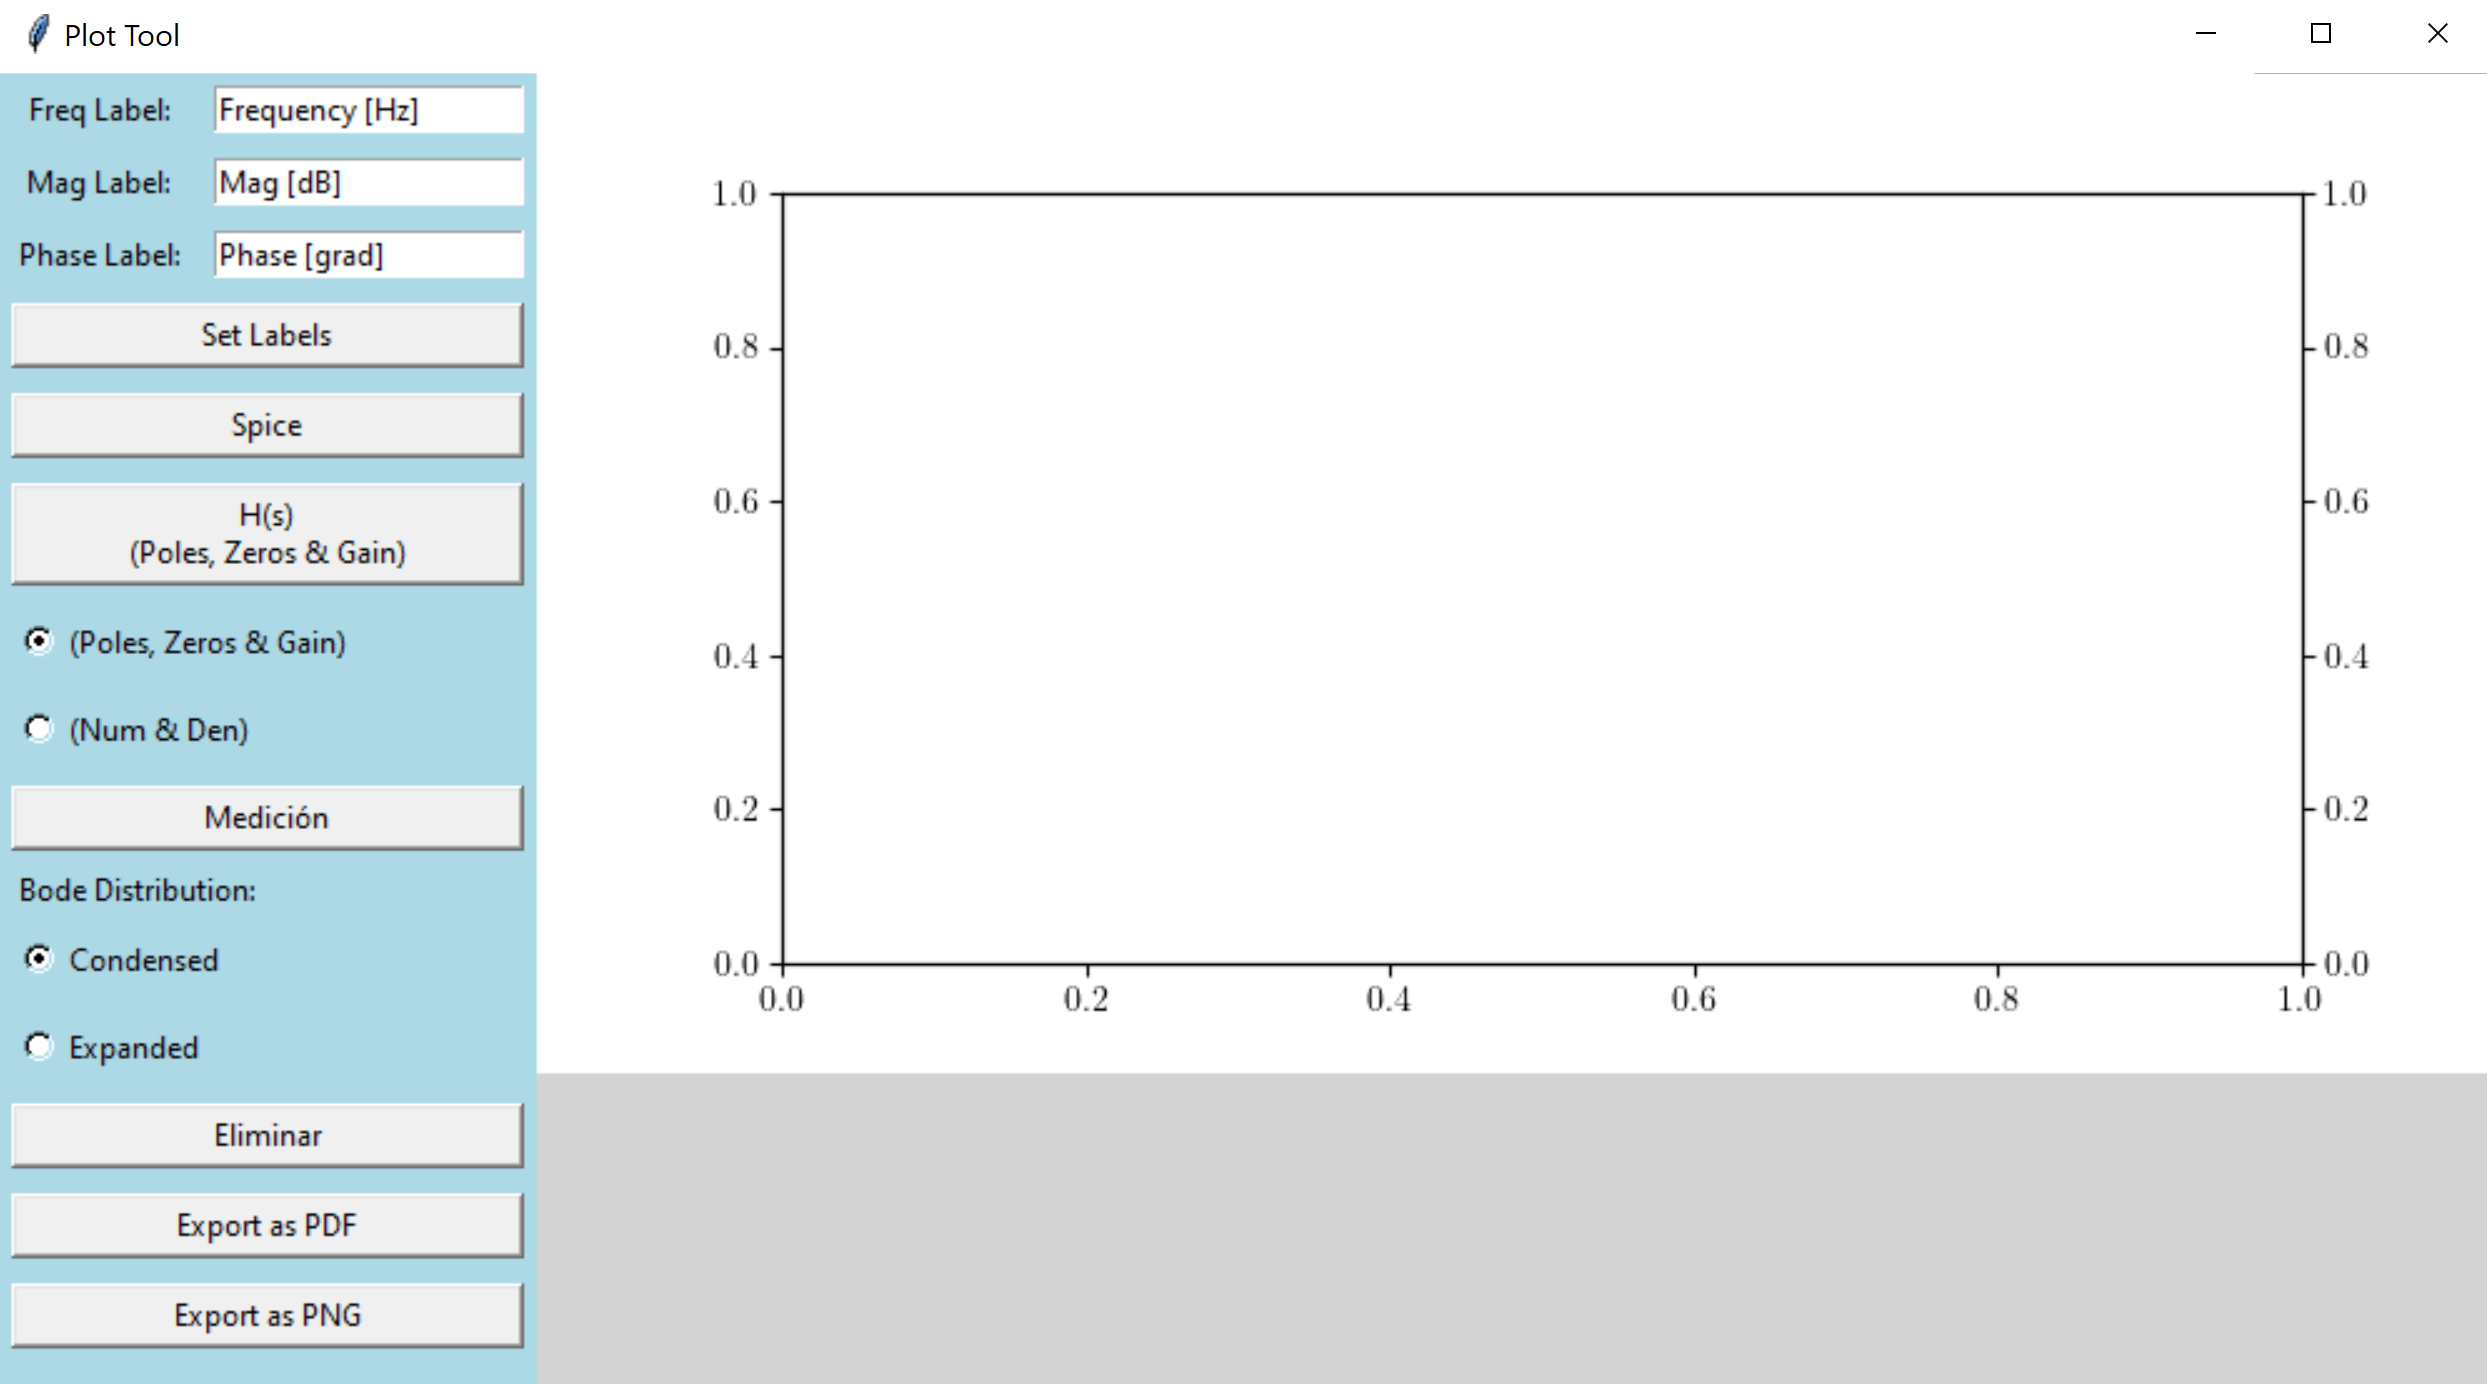
\includegraphics[scale=0.2]{resources/window.png}
\caption{GUI al iniciar el programa}
\label{fig:window}
\end{figure}

A la izquierda se encuentra el panel de controles, cuyo funcionamiento se explicara a continuación, mientras que a la derecha se encuentra la figura donde se graficarán nuestros datos.


\subsubsection{Ingresar datos}
El programa nos permite ingresar datos desde tres fuentes distintas, archivos de LTspice, transferencias analíticas o mediciones(en un formato determinado que se explicara posteriormente). Los tres botones para ingresar los mismos se muestran en la Figura \ref{fig:inputControls}.

\begin{figure}[ht]
\centering
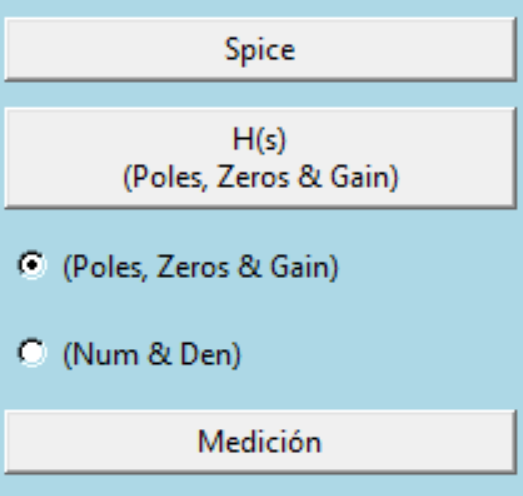
\includegraphics[scale=0.3]{resources/inputControls.png}
\caption{Elementos del panel de controles con referencias}
\label{fig:inputControls}
\end{figure}

El botón 'Spice' abrirá un explorador de archivos, que nos permitirá seleccionar un archivo .txt que previamente habremos exportado desde una simulación de LTspice. El archivo debe corresponder a una simulación del tipo 'AC Analysis', que cuente con la transferencia de un solo nodo. Una vez seleccionado el archivo correspondiente aparecerá el gráfico correspondiente en la figura.

Para ingresar una transferencia analítica contamos con dos posibilidades, puede ser ingresada mediante sus polos, ceros y ganancia ('Poles, Zeros \& Gain') o bien mediante los polinomios del numerador y denominador('Num \& Den'). La opción se selecciona con los controles que se encuentran debajo del boton 'H(s)', y se debe indicar previo a pulsar el botón. 
Si seleccionamos la opción 'Poles, Zeros \& Gain', al pulsar el botón 'H(s)' se abrirá una ventana (Figura \ref{fig:pzgPromt}) en la cual se deben ingresar los datos. El formato de los polos y ceros es el siguiente: suponiendo que la funcion transferencia tiene \emph{n} polos \emph{p1}, \emph{p2}, ... \emph{pn}, se deberan ingresar separados por un espacio: \emph{p1 p2 ... pn}. De la misma forma para los ceros, si la transferencia cuenta con \emph{m} ceros \emph{z1}, \emph{z2}, ... \emph{zm}, se deberán ingresar separados por un espacio: \emph{z1 z2 ... zm}. El campo de la ganancia se llena con el valor de la ganancia correspondiente.

\begin{figure}[ht]
\centering
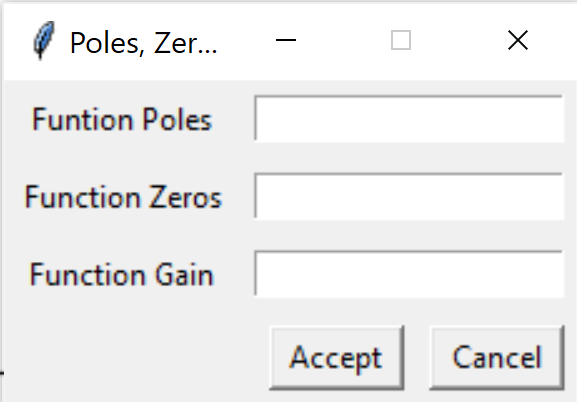
\includegraphics[scale=0.3]{resources/pzgPrompt.png}
\caption{Prompt modo 'Poles, Zeros \& Gain'}
\label{fig:pzgPromt}
\end{figure}

Al seleccionar el modo 'Num \& Den' y pulsar el botón 'H(s)' se abrirá un prompt como el que se muestra en la Figura \ref{fig:numDenPrompt}. Los datos se deben ingresar como un conjunto de coeficientes de polinomios ordenados (estilo polinomio de Matlab). Por ejemplo, si quisieramos ingresar el polinomio $ax^2 + bx + c$, se deberán ingresar los coeficientes \emph{a}, \emph{b} y \emph{c} en forma ordenada separados por un espacio, de la siguiente forma:\emph{a b c}. Los campos Numerador y Denominador admiten el mismo formato.

\begin{figure}[ht]
\centering
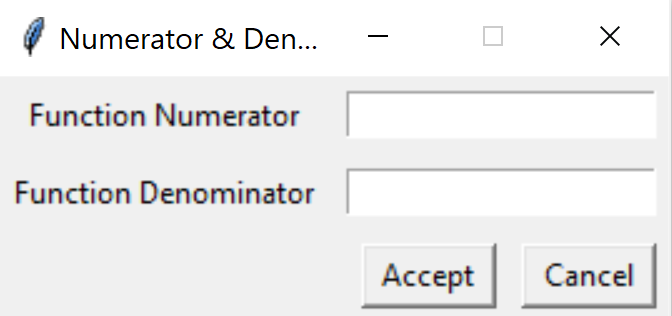
\includegraphics[scale=0.3]{resources/numDenPrompt.png}
\caption{Prompt modo 'Num \& Den'}
\label{fig:numDenPrompt}
\end{figure}

La ultima opción de ingresar datos admite dos tipos de archivos, .csv y .xlsx. El formato de los mismos deberá ser el siguiente:
\begin{itemize}
\item \textbf{.csv: }Los datos deberán contener headers, el caracter de separación de columnas debe ser \emph{;} y el orden de las misma debe ser \emph{frecuencia;magnitud;fase}; frecuencia en Hz, magnitud en dB y fase en grados.
\item \textbf{.xlsx: }Los archivos de Excel deberán estar formateados de la siguiente manera: los datos \emph{frecuencia}, \emph{magnitud} y \emph{fase} deberán colocarse en las columnas A, B y C, respectivamente, el archivo no deben contener headers, y el primer dato deberá colocarse en la fila 0
\end{itemize}

Cada vez que se cargue un dato a graficar, el programa abrirá automáticamente un prompt en el cual se podrá ingresar una etiqueta que describa el gráfico correspondiente.

\subsubsection{Editar etiquetas}

En la parte superior del panel de controles se encuentran tres cuadros de texto en los cuales podemos ingresar las etiquetas de los ejes, como se muestra en la Figura \ref{fig:labesControl}. Por default estas son \emph{Frequency [Hz]}, \emph{Mag [dB]} y \emph{Phase [grad]} para frecuencia, magnitud y fase respectivamente. Para modificarlas, debemos ingresar la etiqueta deseada y hacer click en 'Set Labels'.

\begin{figure}[ht]
\centering
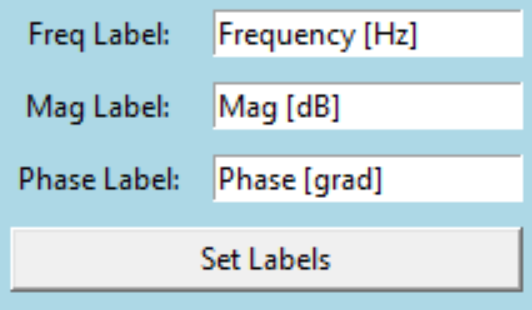
\includegraphics[scale=0.3]{resources/labelsControl.png}
\caption{Controles para modificar etiquetas de ejes}
\label{fig:labesControl}
\end{figure}

\subsubsection{Distribución de los gráficos}
La interfaz cuenta con una herramienta para poder seleccionar la disposición de las curvas. Mediante este control podemos disponer las curvas de magnitud y fase en una misma figura('Condensed'), o separar las curvas de magnitud y fase en dos figuras diferentes('Expanded'). Las Figuras \ref{fig:condensed} y \ref{fig:expanded} muestran los gráficos en modo 'Condensed' y 'Expanded', respectivamente.

\begin{figure}[ht]
\centering
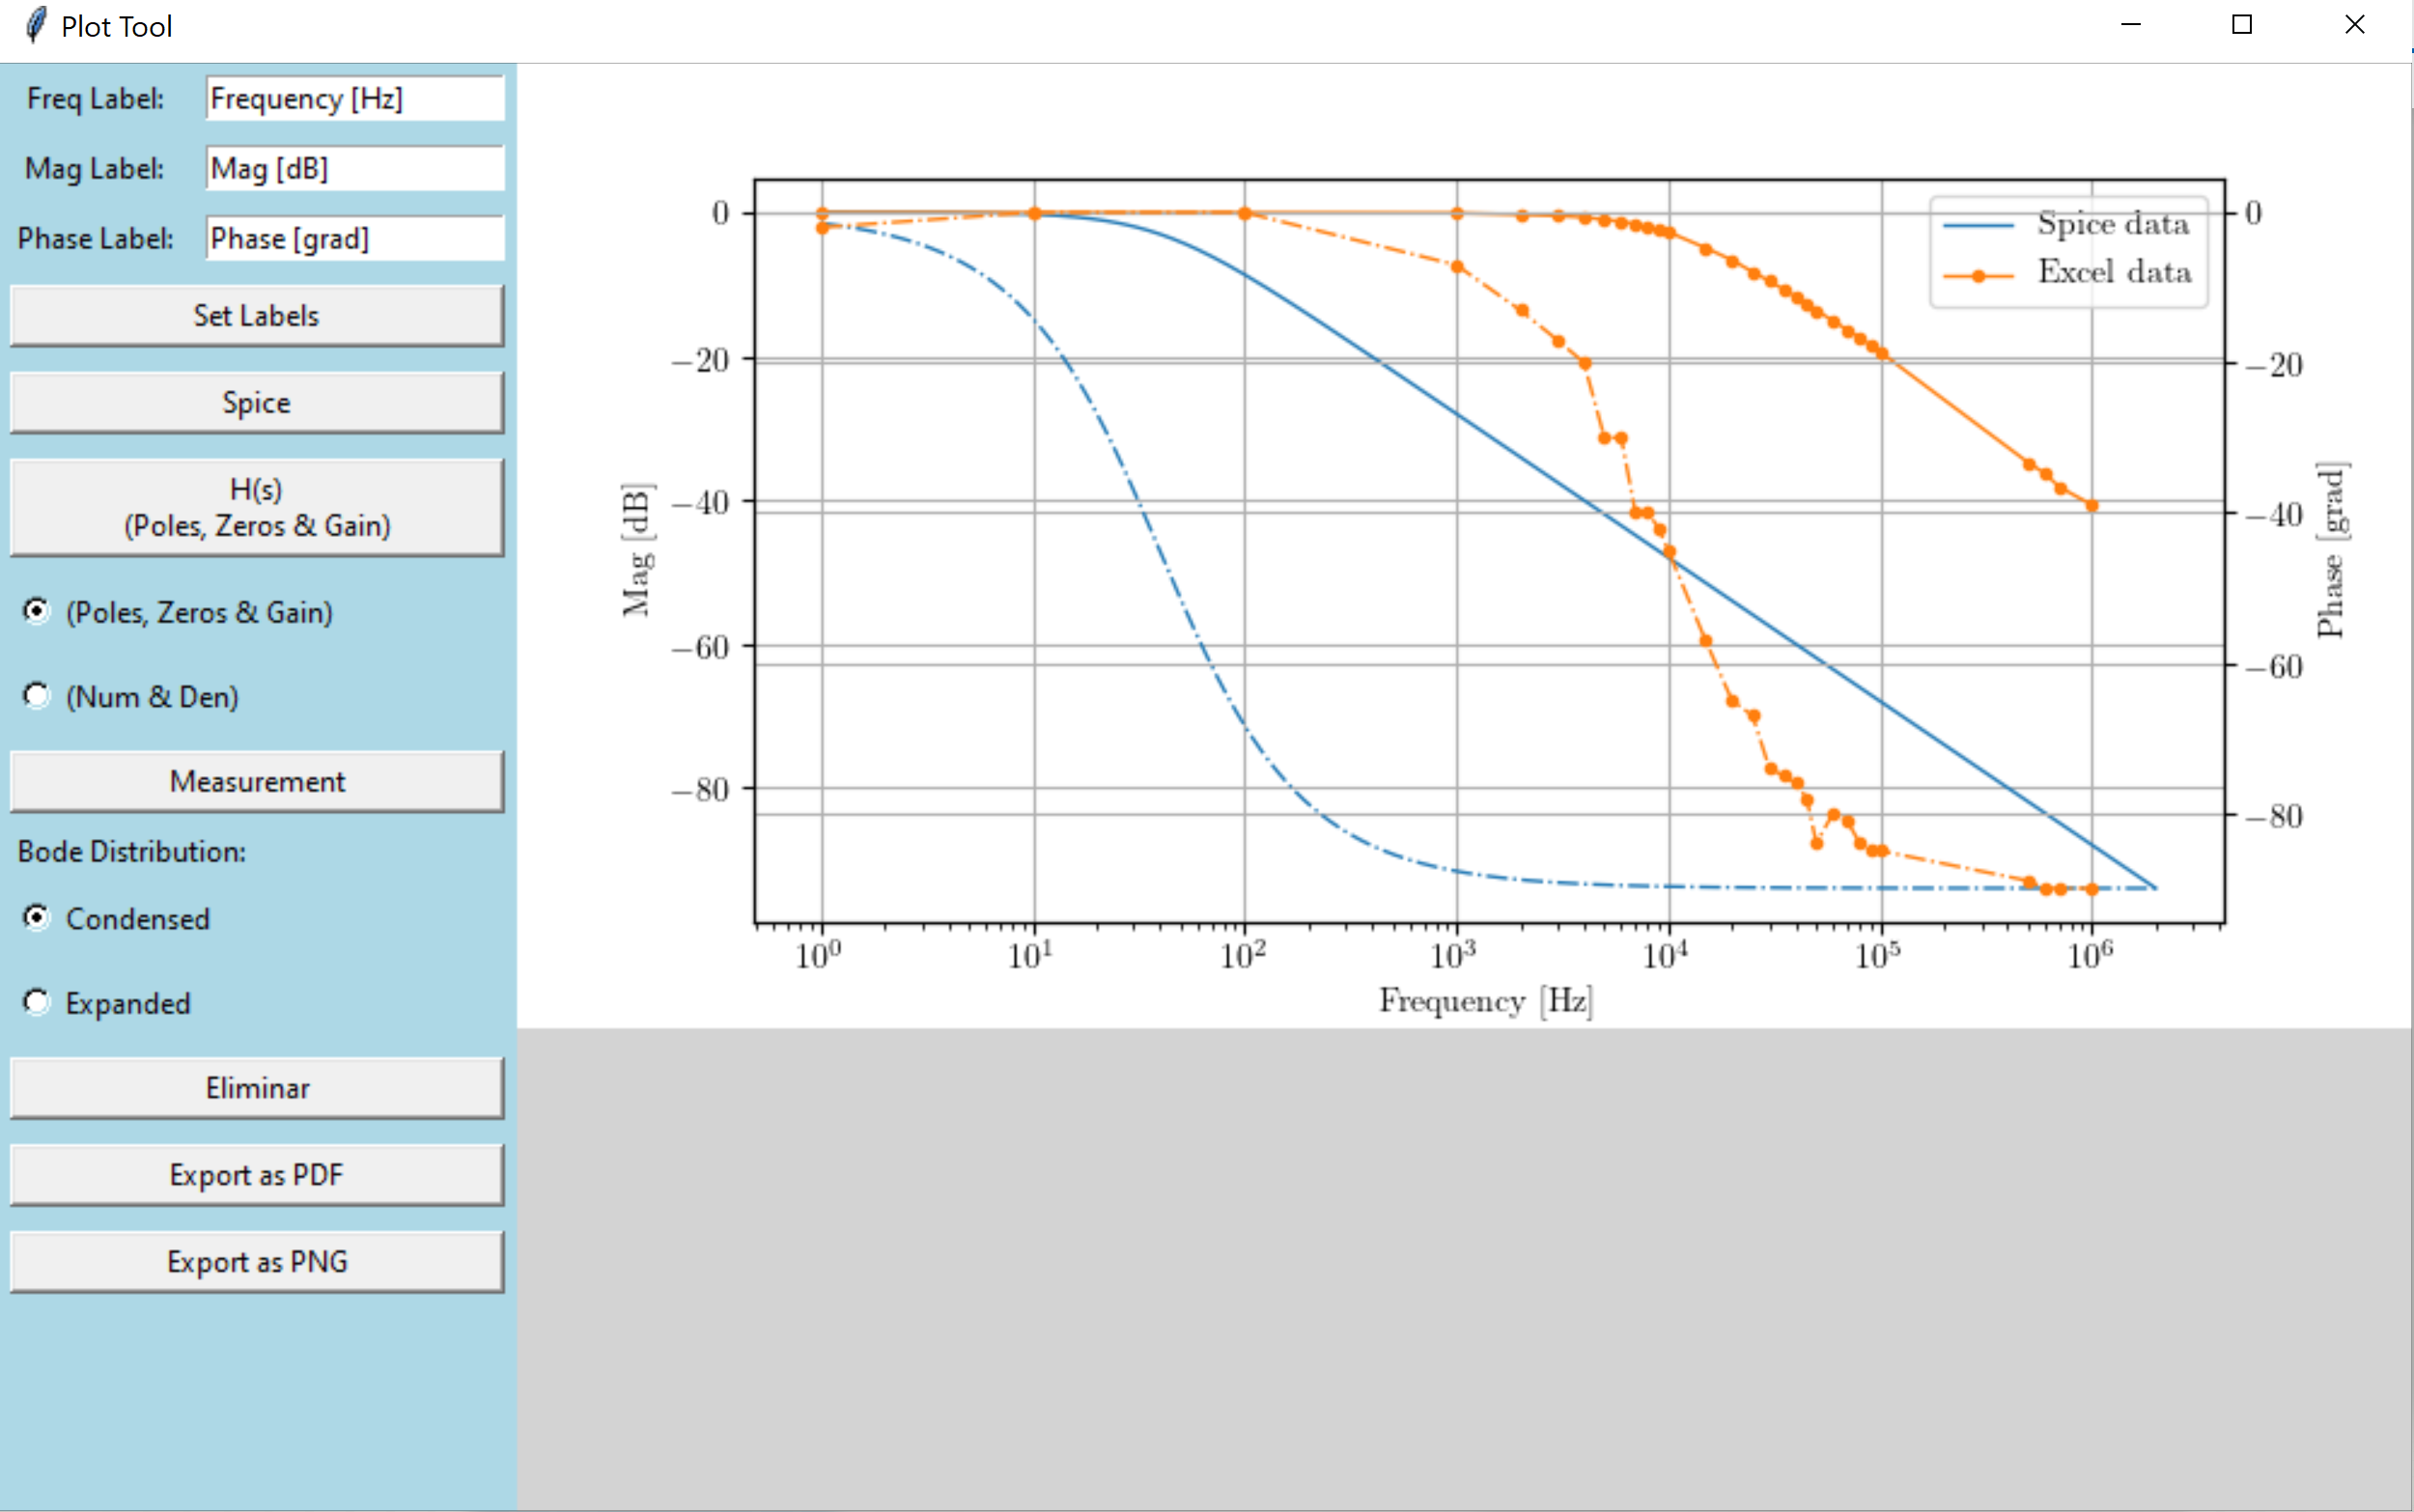
\includegraphics[scale=0.15]{resources/condensed.png}
\caption{Gráficos en modo 'Condensed'}
\label{fig:condensed}
\end{figure}

\begin{figure}[ht]
\centering
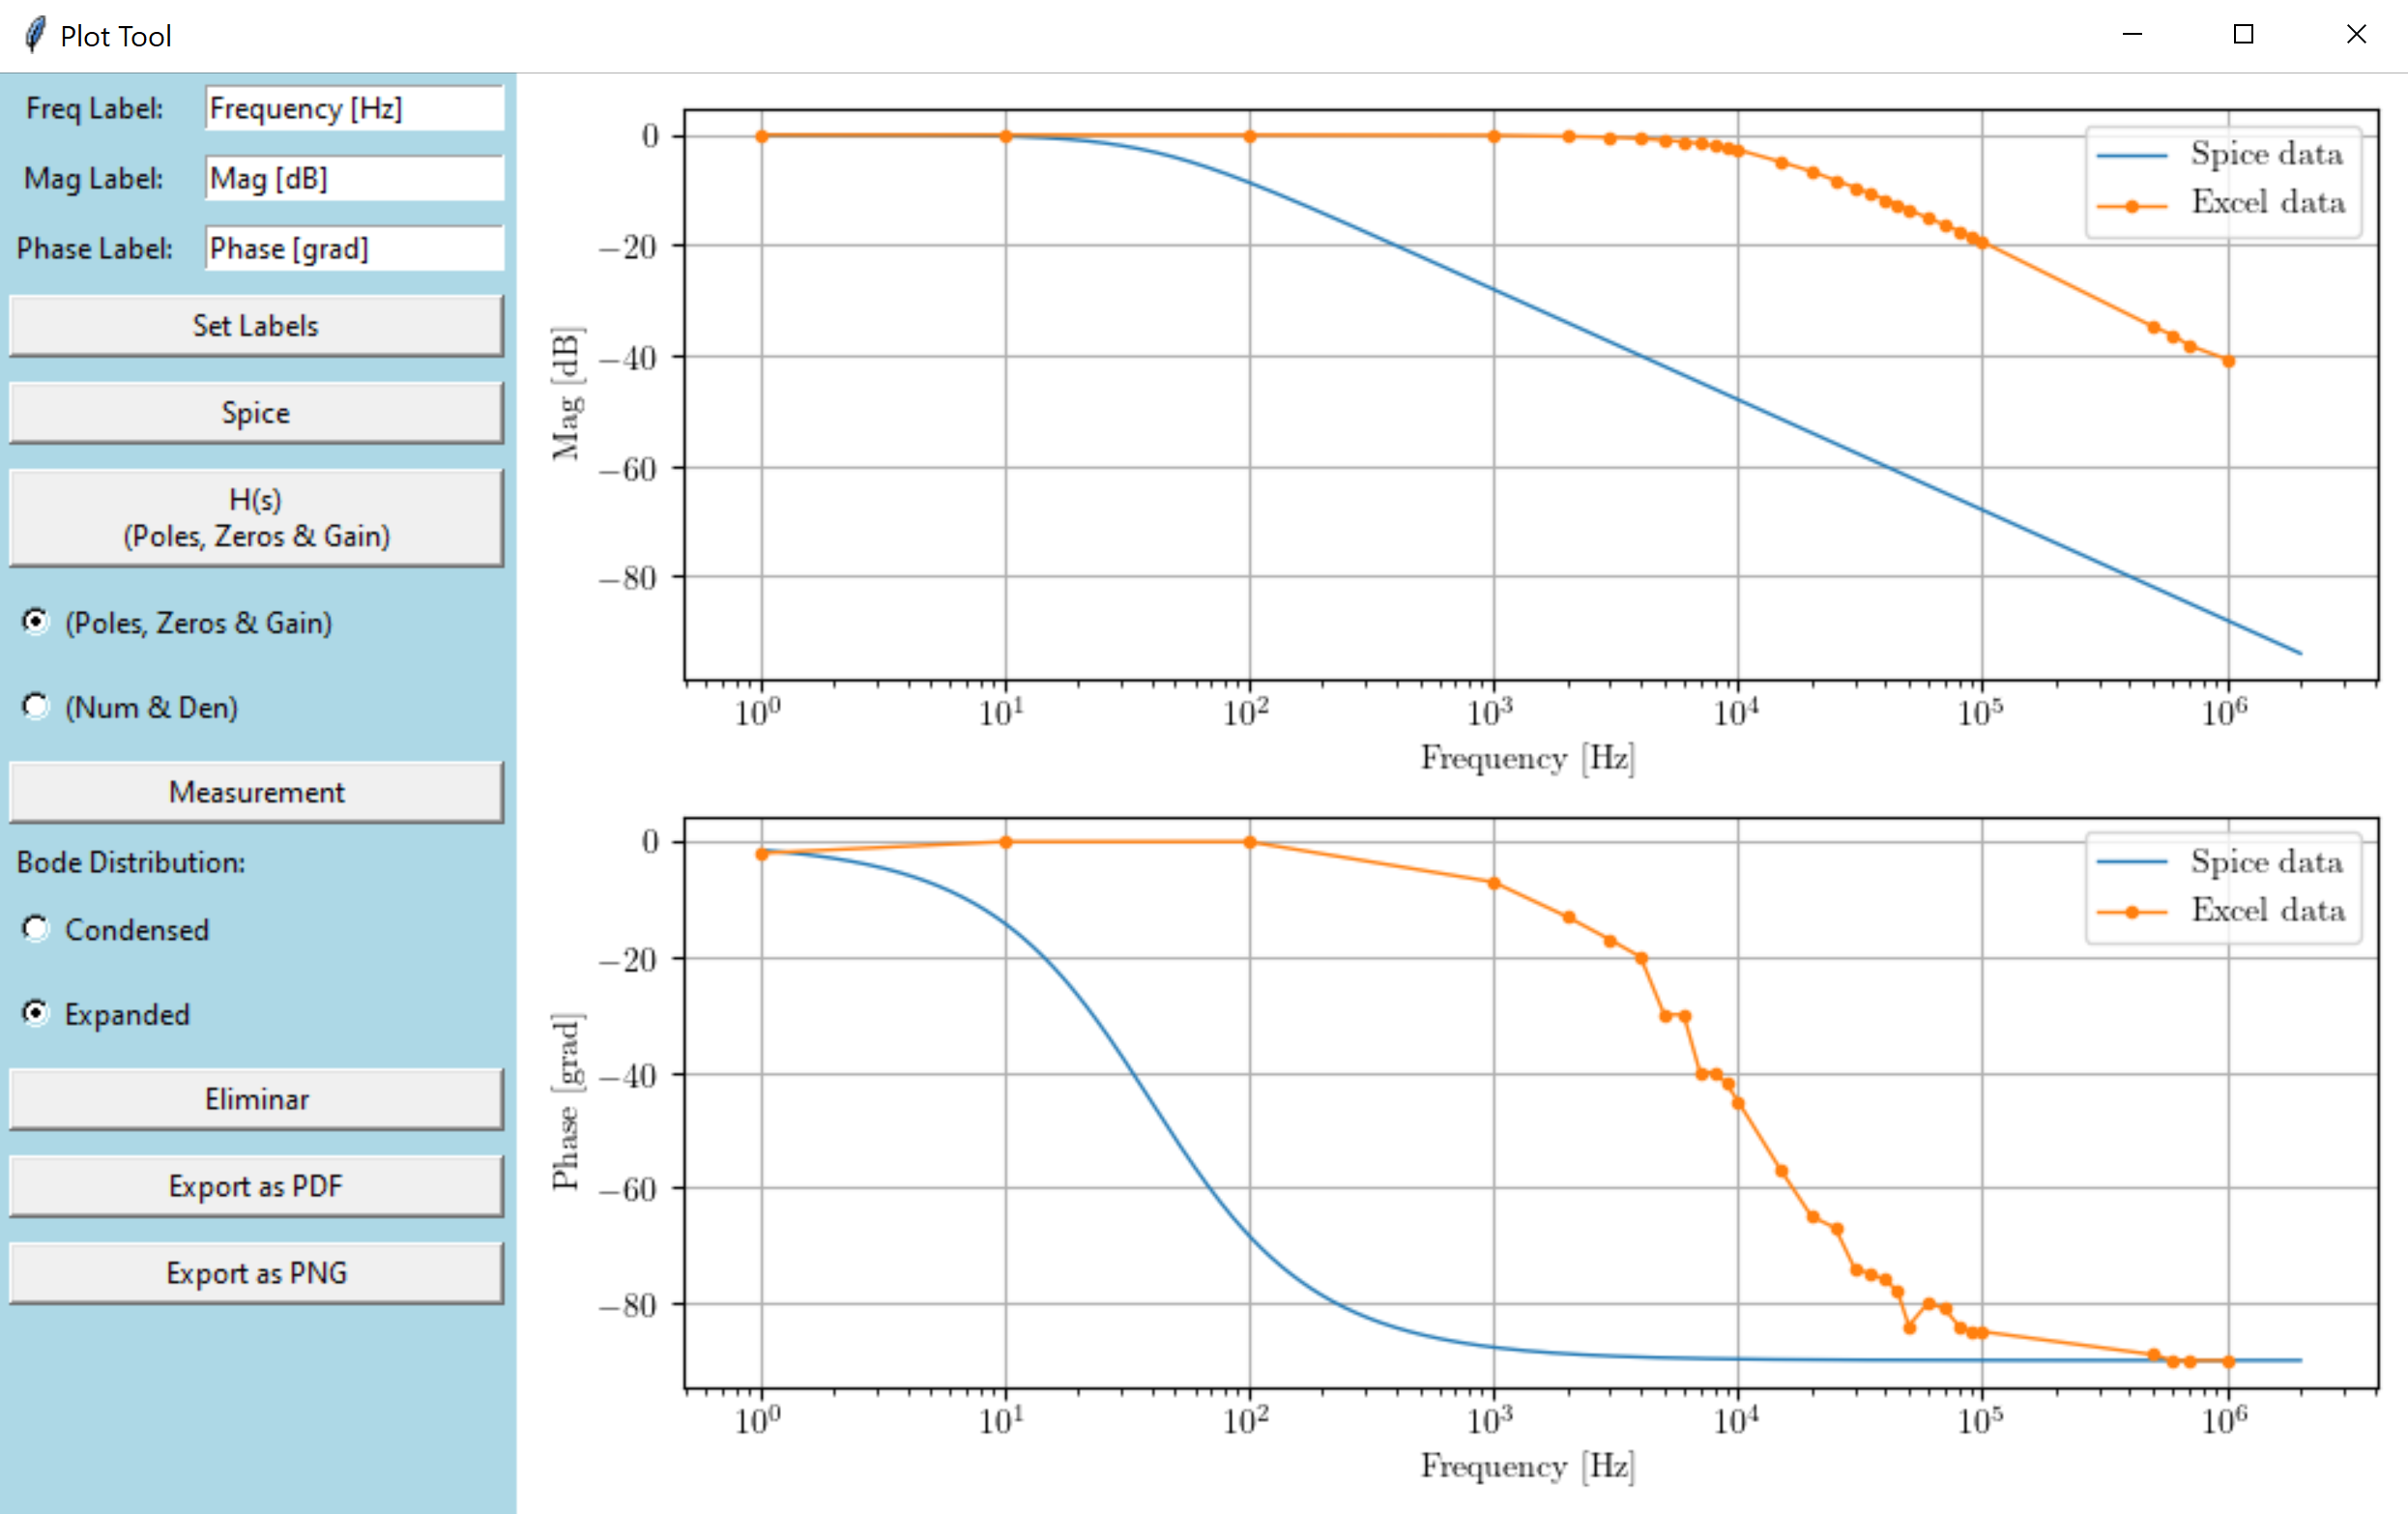
\includegraphics[scale=0.15]{resources/expanded.png}
\caption{Gráficos en modo 'Expanded'}
\label{fig:expanded}
\end{figure}

\subsubsection{Eliminar gráficos}
Para eliminar los gráficos cargados, es necesario hacer click en la opción 'Remove Plots'. Esta herramienta borrará todos los gráficos que estén graficados en la figura. No es posible remover los gráficos individualmente

\subsubsection{Exportar gráficos}
La ultima herramienta de la interfaz permite exportar los gráficos en dos formatos: PDF y PNG. El archivo exportado tendrá el formato que se presente en la GUI según el modo seleccionado (Condensed o Expanded). Al seleccionar el botón de \emph{Exoport as...} se abrirá un explorador de archivos para indicar la ubicación y nombre de nuestro archivo exportado. Las Figuras \ref{fig:condExport} y \ref{fig:expExport} muestran las figuras generadas en ambos modos:

\begin{figure}[ht]
\centering
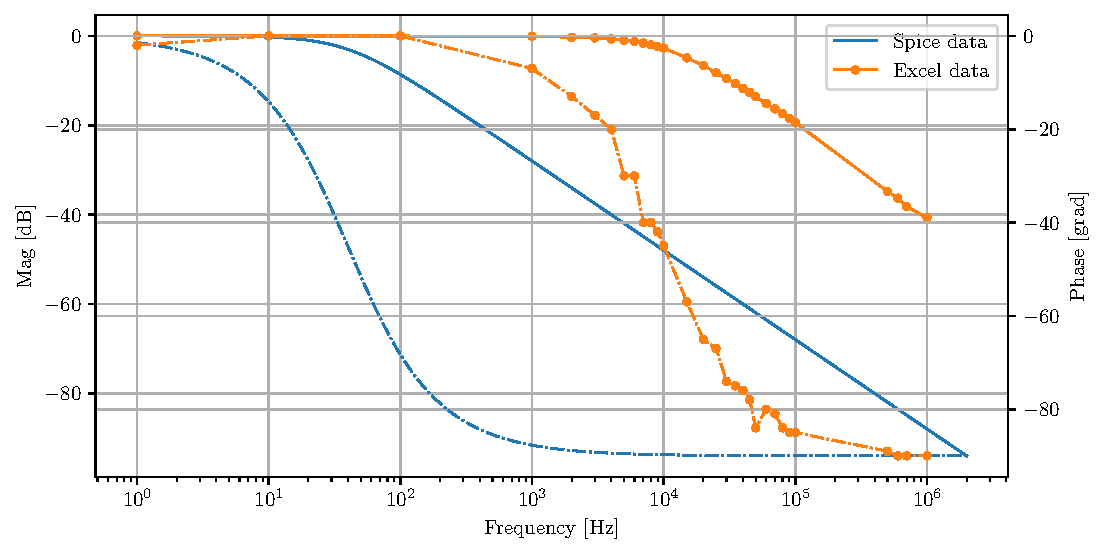
\includegraphics[scale=0.7]{resources/condExport.pdf}
\caption{Resultado exportado en modo 'Condensed'}
\label{fig:condExport}
\end{figure}

\begin{figure}[ht]
\centering
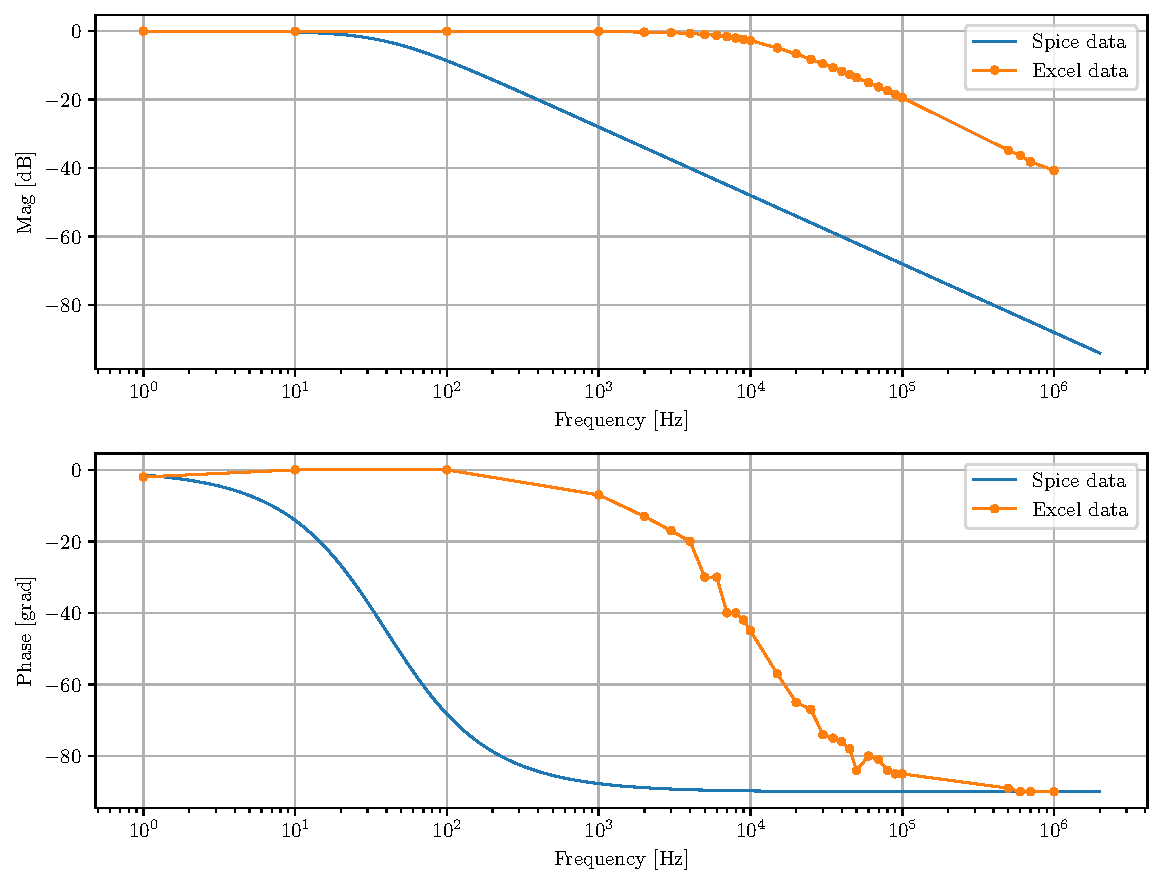
\includegraphics[scale=0.7]{resources/expExport.pdf}
\caption{Resultado exportado en modo 'Expanded'}
\label{fig:expExport}
\end{figure}

\end{document}